\chapter{Developer documentation}
\label{ch:impl}

(0.5)

\section{Architectural Overview}

The toolkit is heavily depends on the libgit2 \cite(libgit2) library which is a portable, pure C implementation  if the Git core methods,
this library has a version for JavaScript and Node.js which is the nodegit \cite(nodegit).
The whole toolkit architecture can be represented with the following diagram:

\begin{figure}[H]
	\centering
	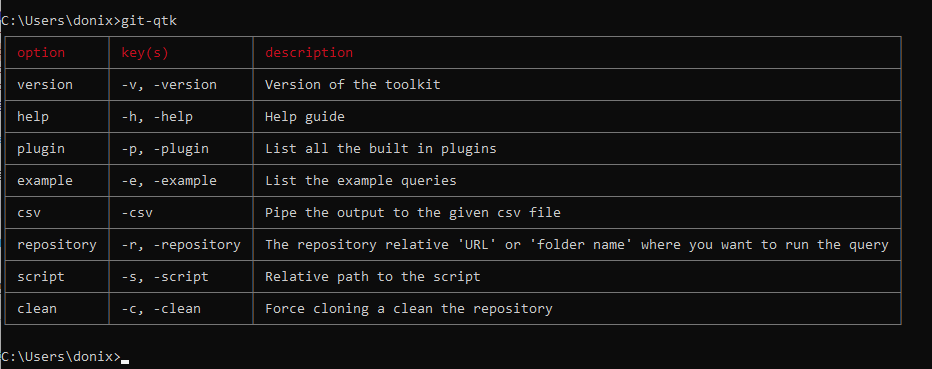
\includegraphics[width=350px]{help}
	\caption{TODO}
	\label{fig:fig-help}
\end{figure}


\subsection{Database}

We need to somehow store all the data coming from the parser and plugins. We can assume that the plugins will reduce the size of the
pure data from the repository history. So to provide maxium performace for the query we can use an in-memory database. 
We can also assume that the database will be immutable after the parsing is done. 

The database is collections of hash maps based on the models. The hash map keys are defined by its model \textit{key()} method.
The reson behind this database structure is in the join mechanism in the query. The hash map is implemeted with the built in 
\textit{Map} \cite{map} which has a acceess time and space compexity of:

\( O(1) \)

In this way if we connect two models where at least of the models field is a key then we can assume that:\newline
N records of the A model, M records of the B model
\(O(N * M) = O(N)\)

\subsection{Extensions}

(2)

\section{Implementations}

(1)

\subsection{Parsing and validating scripts}

(2)

\subsection{Parsing Git histroy}

breadth-first search (2)

\subsection{Running the query}

(2)

\section{Testing}

(0.5)

\subsection{Unit tests}

(2)

\subsection{Integration tests}

(2)

\section{Tools}

(1)

\subsection{Gitub}

\subsection{VS Code}